\documentclass[Screen16to9,17pt]{foils}
\usepackage{zencurity-slides}

\selectlanguage{english}


\usepackage{tabularx}
\usepackage{tikz}
\usetikzlibrary{mindmap,trees}
\usetikzlibrary{shapes.geometric, arrows,automata}
\usetikzlibrary{positioning}

\usepackage{jigsaw}



\tikzset{
    state/.style={
           rectangle,
           rounded corners,
           draw=black, very thick,
           minimum height=2em,
           inner sep=2pt,
           text centered,
           },
}


%\externaldocument{unix-audit-security-oevelser}
\externaldocument{\jobname-exercises}

% Self-hosting og digital suverænitet
% Kun for medlemmer
% Tag kontrollen over dine egne data og bliv uafhængig af Big Tech
% Tag kontrollen over dine egne data og bliv uafhængig af Big Tech

% Vil du gerne være mere uafhængig af store tech-platforme som Google, Microsoft og Amazon, men er i tvivl om, hvor du skal begynde?

% På dette kursus får du en praktisk introduktion til self-hosting og digital suverænitet: hvordan du selv kan drive dine services, styre din infrastruktur og beskytte dine data.
% Vi starter helt fra bunden og gennemgår de vigtigste beslutninger: Skal du hoste hjemme, eller vælge en udbyder ude i verden? Hvilke sikkerhedskrav skal du tage højde for? Og hvad kræver det egentlig at køre sine egne løsninger?

% Vi gennemgår bl.a.:
% * Hvad internettet egentlig består af: IP-adresser, routing og adressering (PI/PA)
% * Hvad du skal overveje, før du hoster dine egne services
% * Fordele og ulemper ved at hoste hjemme
% * Introduktion til VPS, vhosts, containere og Kubernetes
% * Administration og sikring af dit eget miljø
% * Backup og drift af mindre løsninger

% Efter kurset vil du kunne komme i gang med at hoste egne webtjenester og få erfaring med selv at styre infrastrukturen bag. Du får et realistisk overblik over, hvad det kræver, teknisk, praktisk og sikkerhedsmæssigt, at tage kontrollen over dine egne data.

% Nøgleord: hosting, self-hosting, digital suverænitet, infrastruktur, web-løsninger, containere, sikkerhed


\begin{document}


\mytitlepage{Self-hosting and Digital Sovereignty}
{PROSA August 2026}


\hlkprofiluk


\slide{Goals for today}

\hlkimage{7cm}{1984-not-instruction-manual.jpg}

{\bf \large Take control of your own data and become independent of Big Tech}


\begin{quote}\large
Would you like to be more independent of major tech platforms like Google, Microsoft, and Amazon, but aren't sure where to start?
\end{quote}

\slide{AWS: Four Outages in Four Months}
\begin{quote}
Amazon Web Services went down again on Friday morning, July 24, 2026. Around 7:40 a.m. ET, outage trackers lit up with reports that Apple Pay, DoorDash, Reddit, Hulu, and PlayStation Network had all stopped responding at once. The common thread, as AWS and the New York Post both confirmed, was a single AWS region, US-WEST-2 in Oregon, where a regional internet connectivity problem cascaded into a disruption AWS itself would later confirm and, by 9 a.m. ET, resolve.
Kilde: \url{https://tech-insider.org/aws-outage-us-west-2-2026/}
\end{quote}
\begin{list2}
\item May: chiller failure, Northern Virginia -- $\sim$14h recovery
\item June: multi-region disruption tied to network provider Zayo
\item July 24: US-WEST-2 outage takes down Apple Pay, Reddit, Hulu, PSN
\item August: second US-WEST-2 connectivity fault, same network path
\end{list2}

\slide{Danish Municipalities: Sovereignty in Practice}
\begin{quote}{\large \bf
Aarhus Kommune reducerer Microsoft-afhængighed\\
med 25 procent over fire år}

{\bf Byrådet lagde kursen fast med klar procentsats}

Aarhus Byråd traf i efteråret 2025 en konkret politisk beslutning: Over fire år skal kommunen reducere sin afhængighed af Microsofts kontorpakke med 25 procent. Beslutningen gav embedsværket et formelt mandat til at arbejde systematisk med digital handlefrihed og satte dermed gang i et bredere program, der rækker langt ud over kontorpakkens grænser.


Kilde:\\{\scriptsize\url{https://www.lovguiden.dk/det-offentlige/staten-og-kommunernes-indkoebsservice/2026-05-19-aarhus-kommune-reducerer-microsoft-afhaengighed-med-25-procent-over-fire-aar}}
\end{quote}
\begin{list2}
\item Aarhus: whole-stack review, not just office software
\item Aarhus: 25\% open source office software target by 2030
\item Ish{\o}j: only $\sim$50\% of staff now hold a full M365 license
\end{list2}

\slide{Denmark: Sovereignty Reaches the Government Platform}
\begin{quote} {\large \bf
Klumme: Digital suverænitet begynder i udbudsfasen}

Det er ikke nok med gode intentioner og hensigtserklæringer. Digital suverænitet kræver effektive tiltag i stor skala. Vi kan med fordel lade os inspirere af EU.

``Danmark skal ud af sin stavnsbinding til big tech og have større digital selvbestemmelse''\\
-- Morten Kj{\ae}rsgaard, Magenta, ITWatch

Kilde: \url{https://itwatch.dk/Klummer/article19459678.ece}
\end{quote}
\begin{list2}
\item New minister: Christina Egelund (M)
\item ``Digital sovereignty'' mentioned six times in the government platform
\item Political recognition is ahead of concrete follow-through
\end{list2}





\slide{Practical Information}

\begin{quote}
We start from scratch and walk through the most important decisions: Should you host at home, or choose a provider out in the world? What security requirements do you need to consider? And what does it actually take to run your own solutions?
We'll cover, among other things:
\end{quote}


\begin{list2}
\item a practical introduction to self-hosting and digital sovereignty:
\item how to run your own services
\item manage your infrastructure
\item and protect your data.
\end{list2}

Keywords: hosting, self-hosting, digital sovereignty, infrastructure, web solutions, containers, security

BTW Sorry the slides are very text-heavy - hope it helps later, but don't try to read it all!


\slide{Time schedule}

\hlkimage{45mm}{thomas-drouault-IBUcu_9vXJc-unsplash.jpg}


\begin{list2}
\item 17:00 - 18:15 Introduction and basics
\item 30min Break, talk or spend time with family
\item 18:45 - 19:45 Technologies I use and recommend
\item 15min small break
\item 20:00 - 21:00 More open discussion and questions along the way, influence the content
\end{list2}


\slide{My Intentions Today}

\begin{quote}
After the course, you'll be able to get started hosting your own web services and gain hands-on experience managing the infrastructure behind them. You'll get a realistic overview of what it takes -- technically, practically, and from a security standpoint -- to take control of your own data.
\end{quote}

I want to inspire you to change your minds and get started
\begin{list2}
\item What is it?!
\item You are unsure of how to do it
\item My intention is to be your sparring partner today, list the parts I think must be considered.

\item The slideshow can hopefully serve as an inspiration, but maybe also a Warning! -- sometimes let others do the technical stuff \smiley
\end{list2}

\slide{Why are we here today then?!}

\hlkimage{7cm}{eugen-str-CrhsIRY3JWY-unsplash.jpg}

\begin{list2}
\item Identify what we \emph{need} for Self-hosting and Digital Sovereignty
\item Consider more parts of the picture
\item Show solutions that have worked for me, with some example technologies
\item Provide a kind of check list for your deployment
\end{list2}

\slide{Where Does Your Service Run?}

%\hlkimage{}{}

\begin{quote}
From fully managed cloud to bare metal in your own rack —
choosing a hosting model means trading off control, cost, complexity, and trust.
\end{quote}

\begin{list2}
\item {\bf SaaS} — Software as a Service: vendor runs everything, just use it\\
(Gmail, Office 365, Salesforce) — no ops, but no control
\item {\bf PaaS} — Platform as a Service: deploy your code, vendor manages
the runtime, scaling, and OS\\ (Heroku, Render, fly.io)
\item {\bf IaaS} — Infrastructure as a Service: you get virtual machines, you manage
everything above the hypervisor\\ (AWS EC2, Hetzner Cloud, DigitalOcean)
\item {\bf VPS} — a cheap, simple IaaS instance; the typical entry point for self-hosters
\item {\bf On-premises / self-hosted} — your own hardware, your own network,
full control and full responsibility
\item {\bf Hybrid} — mix of the above; e.g.\ data on-prem, compute in the cloud
\item Key questions: Who owns the data? Who is on call at 3am? What is the ongoing cost, price increase next-year, and exit cost?
\end{list2}

\slide{Digital Sovereignty -- Digital suverænitet}

\begin{quote}
Digital suverænitet (også kaldet it-suverænitet, cybersuverænitet) betyder, at aktøren har eksklusiv selvbestemmelse (kontrol) over sine egne data og it-infrastruktur (incl. it-tjenester, datanettet). Med eksklusiv selvbestemmelse menes, at aktøren har de evner og færdigheder, der er nødvendige for at opfylde sine roller autonomt, uafhængigt og sikkert.[1][2]

\begin{list2}
\item Åbne og frie dataformater og digitale grænseflader (incl. APIere).
\item Dataforvaltningsplan - forudsætter skabelse af metadata, der kan sikre at data kan genfindes - og fx anvendes maskinelt.
\item Free/Libre and Open Source Software, FLOSS, FOSS - kan oversættes til "fri og åben-kildekode software". FLOSS's kildekode er let tilgængeligt ("åbent"), og at det kan bruges, ændres og deles frit ("gratis") grundet de anvendte licenser. Dette muliggør aktørens autonomi og uafhængighed.
\item Private cloud - ejes og styres alene af aktøren selv - og private cloud er i samme land som aktøren.
\item Open-source hardware (en) - dvs designet er let tilgængeligt ("åbent"), og at det kan bruges, ændres og deles frit ("gratis").
\end{list2}
\end{quote}

Source: \url{https://da.wikipedia.org/wiki/Digital_suver%C3%A6nitet} - On purpose taking the danish wording


\slide{Self-hosting}

\begin{quote}
Self-hosting is the practice of running and maintaining a website or service, as well as own servers for e-mail, IM, NTP and so on, using a private server, instead of using a service outside of the administrator's own control. Self-hosting allows users to have more control over their data, privacy, and computing infrastructure, as well as potentially saving costs and improving skills.[1][2]
\end{quote}
Source: \link{https://en.wikipedia.org/wiki/Self-hosting_(network)}

\begin{list2}
\item Benefits and Downsides! Which is exactly what we are talking about today
\item Take small steps is my recommendation!
\item What is most important the data, data format, or where it is hosted?
\end{list2}


\slide{What the internet is actually made up of}


\hlkimage{13cm}{how-the-internet-works.jpg}
{\small Source: \emph{How the Internet Really Works
An Illustrated Guide to protocols, privacy, censorship, and governance} by catnip and article 19}\\
\url{https://catnip.article19.org/} {\color{red}\faHeart}
fun and educational book




\slide{What is the Internet}
RFC-1958:
\begin{quote}
 A good analogy for the development of the Internet is that of
 constantly renewing the individual streets and buildings of a city,
 rather than razing the city and rebuilding it. The architectural
 principles therefore aim to provide a framework for creating
 cooperation and standards, as a small "spanning set" of rules that
 generates a large, varied and evolving space of technology.
\end{quote}


\begin{list1}
\item Communication between humans - currently!
\item Based on TCP/IP
\begin{list2}
\item best effort
\item packet switching (IPv6 calls it packets, not datagram)
\item \emph{connection-oriented} TCP
\item \emph{connection-less} UDP
\end{list2}
\end{list1}




\slide{Internet is Open Standards!}

{\hlkbig \color{titlecolor}
We reject kings, presidents, and voting.\\
We believe in rough consensus and running code.\\
-- The IETF credo Dave Clark, 1992.}

\begin{list1}
\item Request for comments (RFC) -- a series of documents spanning decades
\item RFC, BCP, FYI, informational -- first ones from 1969!
\item Are not updated but status is changed to Obsoleted when new versions are published
\item Standards track:\\
Proposed Standard $\rightarrow$ Draft Standard $\rightarrow$ Standard
\end{list1}



\slide{Practical Packet Analysis}


\hlkimage{6cm}{PracticalPacketAnalysis3E_cover.png}

\begin{list2}
\item \emph{Practical Packet Analysis - Using Wireshark to Solve Real-World Network Problems}, 3rd edition 2017, 368 pp\\
Chris Sanders ISBN: 9781593278021
\end{list2}


\slide{OSI Model and Internet Protocols}

\hlkimage{10cm,angle=90}{images/compare-osi-ip.pdf}

\slide{Recommended network technologies to learn}

Small set of recommended networking technologies to learn

Networking: Basic Protocols from the Internet Protocols suite IP/TCP, or TCP/IP
\begin{list2}
\item Network Layer: Ethernet, Address Resolution Protocol (ARP), IPv4 and ICMP\\
Later add Wi-Fi and IPv6
\item Transport Layer: Transmission Control Protocol (TCP) and User Datagram Protocol (UDP)
\item Common upper layer: Dynamic Host Configuration Protocol (DHCP), Domain Name System (DNS),
Hypertext Transfer Protocol (HTTP)\\
Later add the encrypted/secure versions like Hypertext Transfer Protocol Secure (HTTPS) which uses Transport Layer Security (TLS)
\end{list2}

Enough to be able to go to other resources, and a connected path from ARP to TLS

\slide{Public IP address: Provider Aggregatable (PA) Addresses}

\begin{quote}
PA addresses are assigned from an LIR's allocation and are registered in the RIPE Database
by the LIR. The advantage of PA addresses is that the routing information for many customers
can be aggregated once it leaves the provider's routing domain.
\end{quote}
Source: RIPE Network Coordination Centre (RIPE NCC) -- FAQ: ISPs\\
\link{https://www.ripe.net/membership/member-support/faqs/isp-related-questions/pa-pi/}

\begin{list2}
  \item Assigned from a Local Internet Registry's (LIR) own allocation
  \item Registered in the RIPE Database by the LIR itself
  \item Routing information for many customers can be {\bf aggregated} into a single
        announcement, improving global routing efficiency
  \item If an end user changes their upstream provider, the PA addresses
        {\bf must be returned} -- they cannot be taken along
\end{list2}

\slide{Public IP address: Provider Independent (PI) Addresses}

\begin{quote}
PI address space is assigned separately and not from an LIR's PA allocation. All PI
assignments are registered in the RIPE Database by the RIPE NCC at the time they are
assigned. PI assignments are usually small; they cannot be aggregated into larger blocks.
The disadvantage of this is that network operators throughout the Internet may choose
not to route them.
\end{quote}
Source: RIPE Network Coordination Centre (RIPE NCC) -- FAQ: ISPs\\
\link{https://www.ripe.net/membership/member-support/faqs/isp-related-questions/pa-pi/}

\begin{list2}
  \item Assigned {\bf directly by the RIPE NCC} (a Regional Internet Registry),
        not from an LIR's allocation
  \item Registered in the RIPE Database by the RIPE NCC at assignment time
  \item Usually small blocks that {\bf cannot be aggregated} into larger ones
  \item The end user {\bf retains} the address block even when changing ISPs
  \item Network operators across the Internet may choose {\bf not to route} PI
        assignments due to lack of aggregation
\end{list2}

\slide{Current Status IP addresses IPv4 vs IPv6}

\begin{quote}
As the RIPE NCC has run out of IPv4 addresses, no new IPv4 PI address space can be
assigned. IPv6 PI address space is still available.
\end{quote}

\begin{list2}
  \item {\bf IPv4 PI:} No longer available -- RIPE NCC has exhausted its IPv4 pool, can be bought around 20-40USD/IP in chunks of at least 256
  \item {\bf IPv4 PA:} Limited availability -- RIPE NCC has exhausted its IPv4 pool, providers are charging per IP\\
  Usually in Denmark you would get a single public IP for your home connection and enterprise customers can pay for more
  \item {\bf IPv6 PI:} {\bf Still available for assignment through a sponsoring LIR}
  \item {\bf IPv6 PA:} Available through LIR -- but cannot be migrated to new provider!
\end{list2}

So yes, I consider IPv6 a pre-requisite for digital sovereignty!

\slide{IPv6 in Denmark and the EU}

\hlkimage{12cm}{Screenshot_2026-04-21_at_12-06-10_IPv6__Googl.width-1200.png}
\begin{quote}
``Now, 18 years since Google started recording this data, access via
native IPv6 has for the first time exceeded 50\% (50.10\% on 28 March
2026, to be precise).''
\end{quote}
Kilde: \url{https://pulse.internetsociety.org/en/blog/2026/04/18-years-later-ipv6-reaches-majority/}


\slide{The cost of public IP addresses}

\begin{quote}
RIPE NCC members pay an annual contribution (service fee) per Local Internet Registry (LIR). For 2026, this fee is €1,800.

This is charged on a pro rata basis for new members. New members and existing members registering additional LIR accounts also pay a sign-up fee, which is currently €1,000.

Members can have more than one LIR account, but they must pay the membership and sign-up fee for each LIR account. Members also pay €75 per independent assignment or legacy resource and €50 per ASN assignment.
\end{quote}
Source: \link{https://www.ripe.net/membership/payment/}

\begin{list2}
\item The cost involved, get PA would require you to become member of RIPE NCC -- expensive
\item On the other hand! Getting IPv6 PI requires almost nothing, even a person can ask for IPv6 space! Yearly cost would be about EUR 100! This would normally be a /48 IPv6 PI prefix
\end{list2}

Full-disclosure: I have a company that does these requests and charge a yearly fee of €100 -- where €75 is paid to RIPE

\slide{What is a Home Lab}

\begin{quote}
"A homelab is a self-contained IT environment that you design and control. It usually includes basic infrastructure like compute, storage, and networking, along with a hypervisor or virtualization layer. Some setups are modest and run on a single machine, while others resemble mini datacenters with multiple nodes and shared storage such as SAN or NAS."
\end{quote}
Source: StorMagic, "What Is a Homelab? Why IT Pros Are Building Their Own" (stormagic.com, 2025)

\begin{list2}
\item it's your own private sandbox -- no stakes
\item no risk to production systems
\item where you can freely experiment with servers, networking, virtualization, security tools,
\item and anything else you're curious about
\item I think that doing any kind of experiment, then you \emph{have a lab}
\end{list2}

Note: yes, you can run your services at home, but I definitely prefer hosting things outside of my home!

\slide{Hosting at Home: Pros}

\begin{list2}
\item Full control and privacy -- data stays on hardware you own, with no third party scanning or selling it
\item Cost savings over time -- after upfront hardware costs, no ongoing expenses or monthly SaaS fees
\item Deep customization -- configure every service exactly as you want, with no vendor-imposed limitations
\item Upgrade to new versions when you want to, or not if you like the long term stable version
\item No vendor lock-in -- immune to price hikes, shutdowns, or feature removals by external providers
\item Learning technologies -- hands-on experience with networking, Linux, and server security
\end{list2}


\slide{Hosting at Home: Cons}

\begin{list2}
\item If using IPv4 -- you only have one IP, IPv6 may or may not be available
\item Reliability risk -- home power lack data-centre-grade battery backup (UPS)
\item Security burden -- misconfigured or unpatched services exposed to the internet can put your whole network at risk
\item Email delivery is hard -- residential IPs are often blocklisted; SPF/DKIM/DMARC setup is non-trivial
\item ISP restrictions -- port 25 blocking and dynamic IPs complicate running mail or web servers
\item You have a crap router on home connections, even on fiber connections with 1Gbps!
\item No built-in redundancy -- hardware failure, fire, or flood can mean permanent data loss without disciplined offsite backups
\end{list2}


\slide{Operating Systems}

Computers need software -- operating systems, and applications run on an OS:
\begin{list2}
\item OS is the base for your experiments
\item Must be managed, installed at least, updated and packages installed on top
\item Some applications need a regular OS, others are fine with containers
\item Some applications like Python can even use a virtual environment
\end{list2}

TL;DR you need even more skills, sorry!


\slide{Virtualisation}

Computers can run multiple operating systems, and OS distributions at the same time:
\begin{list2}
\item Full virtual machine virtualisation
\item Containers -- including containers platforms like Kubernetes
\item Use it, and create many virtual machines/containers
\item Switch context easily, one project - one (or more) VMs
\item Create a new VM in seconds -- keep one template VM updated that you can clone
\item Install crap -- delete a VM, retry
\item Performance of VMs and containers on modern CPUs is great! Almost like having two physical computers!
\end{list2}

Good news, you can do it all in a single PC! Even a small one!


\slide{Virtualization}

\hlkimage{20cm}{containers.png}

\slide{Example software for virtualisation}

%\hlkimage{ cm}{ }
\begin{list2}
  \item {\bf KVM} (Kernel-based Virtual Machine) -- Linux kernel hypervisor, often managed via libvirt/virt-manager
  \item {\bf Proxmox VE} -- Open-source platform combining KVM and LXC containers, very popular for home labs
  \item {\bf Microsoft Hyper-V} -- Built into Windows Server and Windows 10/11 Pro, easy entry point for Windows users
  \item {\bf VirtualBox} -- Free, cross-platform Type-2 hypervisor by Oracle, great for desktop-level home labs
  \item {\bf VMware ESXi} -- Enterprise-grade Type-1 hypervisor with a free tier (though licensing has changed under Broadcom)
  \item {\bf XCP-ng} -- Open-source fork of Citrix Hypervisor (XenServer), managed via Xen Orchestra
\end{list2}

I use KVM for labs and production, you need to evaluate which one to use

\slide{Virtual Private Servers (VPS)}

\begin{list2}
\item A VPS is a virtualised slice of a physical server, giving you dedicated CPU, RAM, and storage
\item Runs its own full operating system -- you have root access and full control over the environment
\item Provided by hosts such as DigitalOcean, Linode, and Hetzner at low monthly cost
\item Ideal for hosting websites, mail servers, and small applications with predictable traffic
\item Scales vertically by upgrading the plan, but requires manual intervention to resize
\item Similar to running a virtual machine on your laptop
\item Full system administration, like Debian \verb+apt update; apt upgrade+
\end{list2}

Note: the three vendors listed have been used by my customers, and is not a recommendation per se.\\ Evaluate options carefully for yourself


\slide{Containers}

\hlkimage{11cm}{containers_only.png}

\begin{list2}
\item Containers package an application and all its dependencies into a single portable unit
\item Share the host OS kernel -- lighter and faster to start than full virtual machines
\item Docker is the dominant developer-facing tool; images are built from a \verb+Dockerfile+ and stored in registries
\item Images are not Docker-specific -- the industry standard is the {\bf OCI image format}, supported by all modern tools
\item {\bf Compose files} allow multi-container applications (e.g.\ app + database) to be defined and run together
\item Pre-packaged systems that require less administration -- {\bf only configuration}
\end{list2}


\slide{Container Standards and Runtimes}

\begin{list2}
\item The {\bf Open Container Initiative (OCI)} defines three open standards:\\
image-spec, runtime-spec, and distribution-spec \link{https://opencontainers.org}
\item Any OCI-compliant image can be built with one tool (e.g.\ Buildah, Docker) and run with another -- no vendor lock-in
\item {\bf runc} is the reference low-level runtime implementing the OCI runtime-spec; most runtimes use it under the hood
\item Kubernetes communicates with runtimes via the {\bf Container Runtime Interface (CRI)} -- a gRPC-based plugin API
\item {\bf containerd} and {\bf CRI-O} are the two main CRI-compliant runtimes; Docker's direct integration was removed in Kubernetes v1.24 \link{https://kubernetes.io/docs/setup/production-environment/container-runtimes/}
\item CRI-O is purpose-built for Kubernetes -- lightweight, OCI-compliant, and the default in Red Hat OpenShift \link{https://cri-o.io}
\end{list2}


\slide{Kubernetes}

\begin{list2}
\item Kubernetes (K8s) is an open-source system for automating deployment and management of containers at scale
\item Organises containers into \textit{Pods}, grouped by \textit{Deployments}, and exposed via \textit{Services}
\item Provides automatic scaling, self-healing, and rolling updates with zero downtime
\item Suited to large, complex microservice architectures -- significant operational overhead for small projects
\item Managed offerings (GKE, EKS, AKS) reduce setup burden but increase cloud dependency
\end{list2}

\slide{Virtual Hosts in Web Servers}

\begin{list2}
\item Virtual hosting allows a single server or IP address to serve multiple websites or domains
\item Configured at the web server level -- supported natively by both Apache and Nginx
\item Name-based virtual hosting uses the HTTP Host header to route requests to the correct site
\item Efficient use of resources: one system can host dozens of sites with minimal overhead
\item Essential technique for shared hosting environments and multi-tenant web servers
\end{list2}

Side note: Digital Ocean and NGINX as a reverse proxy

That said DigitalOcean has very good documentation for lots of things! example:\\
\link{https://www.digitalocean.com/community/tutorials/how-to-configure-nginx-as-a-reverse-proxy-on-ubuntu-22-04}

\slide{Summary: Technology Comparison}

\begin{center}
\begin{tabular}{|l|l|l|l|}
\hline
{\bf Technology} & {\bf Best For} & {\bf Complexity} & {\bf Scalability} \\
\hline
VPS              & Single apps, full OS control   & Low    & Vertical (manual)   \\
Containers       & Portable, consistent deploys   & Medium & Horizontal (manual) \\
Kubernetes       & Large-scale microservices      & High   & Horizontal (auto)   \\
Virtual Hosts    & Multi-site on one server       & Low    & Limited             \\
\hline
\end{tabular}
\end{center}

\begin{list2}
\item Above does not consider if you are a private person running systems for yourself, friends, family
\item If you are a company with a few services
\item If you are a large company that want to switch over to something privately owned
\item Above are in my opinion good options for running your complete infrastructure!
\end{list2}


\slide{NGINX as a Reverse Proxy}

\hlkimage{10cm}{nginx_reverse_proxy.png}
\begin{list2}
\item A reverse proxy sits in front of backend servers, accepting client requests and forwarding them internally
\item NGINX uses the \verb+proxy_pass+ directive to route traffic to upstream services by hostname or IP
\item Enables virtual hosting -- one public IP can serve many backend applications on different domains
\item Provides TLS termination, load balancing, caching, and request buffering at the edge\\
A single system with NGINX get certificates with Let's Encrypt (or alternatives)
\item Backend servers remain hidden from the public internet, improving security and flexibility
\end{list2}

% \link{https://en.wikipedia.org/wiki/Reverse_proxy}




\slide{Administration and securing your own environment}


Defense in depth

%\hlkimage{10cm}{Bartizan.png}
\hlkimage{13cm}{medieval-clipart-5}
\centerline{Picture originally from: \url{http://karenswhimsy.com/public-domain-images}}


\slide{Firewalls}

\hlkimage{8cm}{opal-luci-firewall-easy.png}

\begin{list2}
\item Firewalls are a great project to look into, there are so many \smiley
\item I recommend looking into open source firewalls like OPNsense, UFW and OpenBSD and many routers also include firewalls. You can often find images from commercial vendors, that you can try out.
\end{list2}


\slide{Firewall OPNsense GUI based and easy to install}

\hlkimage{12cm}{images/screenshots_OPNsense-1024x518.png}

\begin{list2}
\item OPNsense \link{https://opnsense.org/}
\item Firewall built on FreeBSD with web interface
\item Originally thoughts from m0n0wall and later \link{https://www.pfsense.org/}\\
\item Danish companies have been using these for many years now
\end{list2}


\slide{Linux Uncomplicated Firewall (UFW)}

Debian / Ubuntu:
\begin{alltt}\scriptsize
root@debian01:~# apt install ufw
...
root@debian01:~# ufw allow 22/tcp
Rules updated
Rules updated (v6)
root@debian01:~# ufw enable
Command may disrupt existing ssh connections. Proceed with operation (y|n)? y
Firewall is active and enabled on system startup
root@debian01:~# ufw status numbered
Status: active

     To                         Action      From
     --                         ------      ----
[ 1] 22/tcp                     ALLOW IN    Anywhere
[ 2] 22/tcp (v6)                ALLOW IN    Anywhere (v6)
\end{alltt}

\begin{list2}
\item Extremely easy to use -- I recommend and use the (Uncomplicated Firewall) UFW
\item Perfect for a VPS, virtual server somewhere
\end{list2}


\slide{Together with Firewalls - Virtual LAN (VLAN)}

\hlkimage{8cm}{vlan-portbased.pdf}

\begin{list1}
\item Managed switches often allow splitting into zones called virtual LANs
\item Most simple version is port based
\item Like putting ports 1-4 into one LAN and remaining in another LAN
\item Packets must traverse a router or firewall to cross between VLANs
\end{list1}

\slide{Virtual LAN (VLAN) IEEE 802.1q}

\hlkimage{16cm}{vlan-8021q.pdf}

\begin{list1}
\item Using IEEE 802.1q  VLAN tagging on Ethernet frames
\item Virtual LAN, to pass from one to another, must use a router/firewall
\item Allows separation/segmentation and protects traffic from many security issues
\end{list1}

\slide{Network Segmentation: Which VLANs to create}

Using VLANs to segment networks we can extend it to the rest of the network, and an example of isolated segments could be:
\begin{list2}
\item Guest network for cabled and Wi-Fi clients
\item Client networks can be isolated per department, floor or building
\item Server networks for multiple purposes – development, staging, testing, production, manufacturing, …
\item Internet servers in a demilitarized zone (DMZ) which would make it less likely that compromised internet
server would affect the rest of the network
\item Dedicated printer network
\item Management network for virtualisation, one for network management, one for storage
\end{list2}



\slide{Proxy servers and Web Application Firewalls (WAF)}

\begin{list2}
\item Filtering at higher layers is also possible
\item Web proxies for clients can help security a lot -- a centralized filter for everyone

\item Reverse proxies for web applications are called
Web Application Firewalls (WAF) -- and filter incoming web requests, and outgoing answers. Can help with attacks like SQL injection and exfiltration of data
\item Depending on your network it can replace or be combined with filtering on DNS servers, and I would prefer to filter domains with DNS
\item I would also prefer blocking large prefixes of IP destinations using routers/stateless packet filters -- maybe use BGP for distributing \emph{lists}
\end{list2}

Also great home lab projects!

\slide{Example, Restricting the Kubernetes API}

%\hlkimage{}{}

Watch out when learning, you may expose an \emph{admin interface}
\begin{quote}{\bf
By default, the Kubernetes API server listens on port 6443 on the first non-localhost network interface, protected by TLS}. In a typical product
ion Kubernetes cluster, the API serves on port 443. The port can be changed with the --secure-port, and the listening IP address with the --bind
-address flag.

...

If your cluster uses a {\bf private certificate authority, you need a copy of that CA certificate configured into your ~/.kube/config on the cli
ent}, so that you can trust the connection and be confident it was not intercepted.
\end{quote}

\begin{list2}
\item If an attacker can run Kubectl with credentials -- they can do anything
\item Defense in Depth is suggested -- so restrict at multiple levels
\item Only allow connections from specific network -- firewall filtering
\item Use TLS and verify/copy certificates
\end{list2}

\slide{CrowdSec -- Crowd sourced security information}

%\hlkimage{}{}

\begin{quote}
{\bf Detect and block Log4j exploitation attempts with CrowdSec}\\
If you work in Infosec, you had a very lousy weekend. And that’s because of the Log4j zero-day vulnerability (CVE-2021-44228) that was discovered. We had no cho
ice but to roll up our sleeves to help our community before things got messier than they already were.

As a result, we have released a scenario that will help you detect and block exploitation attempts of the vulnerability. This new scenario can be directly downl
oaded from our Hub and installed in a blink of an eye. Check this quick video to see the plugin in action:
\end{quote}

\url{https://www.crowdsec.net/blog/detect-block-log4j-exploitation-attempts}


\begin{list2}
\item Log4j is a popular software library in the Java world
\item CrowdSec quickly provided a list of systems scanning the internet for this vulnerability\\
 \link{https://gist.github.com/blotus/f87ed46718bfdc634c9081110d243166}
\item Full disclosure they gave me a hoodie at an event \smiley
\end{list2}


\slide{CrowdSec with NGINX}

%\hlkimage{8cm}{crowdsec_nginx.png}

\begin{list2}
\item {\bf CrowdSec} is an open-source, community-driven security engine -- the llama company \link{https://crowdsec.net}
\item {\bf NGINX Bouncer} -- a Lua plugin enforcing ban decisions in real time via \verb+access_by_lua_block+,
blocking malicious IPs before requests reach the backend
\item {\bf Security Engine} -- reads NGINX logs and detects behavioural patterns: HTTP probing,
scanning, brute force, and matches against the community blocklist
\item {\bf AppSec/WAF component} -- inline virtual patching, SQLi, XSS, and known CVE protection;
install with:
\verb+cscli collections install crowdsecurity/appsec-virtual-patching+
\item {\bf Community Blocklist} -- crowd-sourced IP reputation feed, continuously updated from
millions of sensors worldwide; free tier available
\item Two complementary modes: reactive (log-based, bans offenders) and
inline (WAF, blocks the request before it is processed)
\end{list2}
Source: Docs: \link{https://docs.crowdsec.net/u/bouncers/nginx/}




\slide{Backup and Operations }

A few sample KVM-Specific Backup Tools
\begin{list2}
  \item {\bf Proxmox Backup Server (PBS)} -- Dedicated backup server for Proxmox/KVM environments. Supports deduplication, compression, and incremental backups.
  \item {\bf Virt-backup} -- Lightweight Python tool for backing up libvirt/KVM virtual machines. Simple and scriptable.
  \item {\bf Restic} -- Fast, secure, and deduplicated backups. Supports local, SFTP, S3, and many other backends.
  \item {\bf Borg Backup} -- Deduplicating archiver with compression and encryption. Often paired with Borgmatic for automation.
  \item {\bf Duplicati} -- Web UI-based backup tool with support for cloud storage backends. Good for beginners.
  \item {\bf Bacula} -- Enterprise-grade, client-server backup system. Very flexible but complex to configure.
  \item {\bf Rsync} -- The classic file sync and backup tool. Often used in scripts for simple home lab backups.
\end{list2}


\slide{Infrastructure as code}

%\hlkimage{}{}

\begin{quote}
{\bf Infrastructure as code (IaC)} is the process of managing and provisioning computer data centers through machine-readable definition files, rather than physical hardware configuration or interactive configuration tools.[1] The IT infrastructure managed by this comprises both physical equipment such as bare-metal servers as well as virtual machines and associated configuration resources. The definitions may be in a version control system. It can use either scripts or declarative definitions, rather than manual processes, but the term is more often used to promote declarative approaches.
\end{quote}
Source: {\footnotesize
\link{https://en.wikipedia.org/wiki/Infrastructure_as_code}}

\begin{list2}
\item Has become the norm in many places
\item I use mostly Ansible to automate \emph{system administration}
\item I highly recommend using version control from the beginning! Use Git to store
\end{list2}


\slide{Docker Compose as Infrastructure as Code}

%\hlkimage{}{}

\begin{quote}
{\bf Docker Compose} is a tool for defining and running multi-container applications
using a declarative YAML file — \verb+docker-compose.yml+. The entire application stack,
including services, networks, volumes, and environment configuration, is described
in a single file that can be version-controlled, reviewed, and reproduced identically
on any machine with Docker installed.
\end{quote}

Source: {\footnotesize
\link{https://docs.docker.com/compose/}}

\begin{list2}
\item A Compose file defines {\bf services} (containers), {\bf networks}, and {\bf volumes} declaratively
\item Running \verb+docker compose up+ brings up the entire stack — no manual steps
\item Files live in version control alongside application code — changes are auditable
\item Ideal for development environments, CI pipelines, and simple self-hosted deployments
\item Compose files are valid IaC: they are machine-readable, repeatable, and diff-able
\end{list2}


\slide{Kubernetes as Infrastructure as Code}

%\hlkimage{}{}

\begin{quote}
{\bf Kubernetes} manages containerised workloads through declarative YAML manifests.
Rather than issuing imperative commands, operators describe the {\bf desired state}
of the cluster — deployments, services, ingress rules, storage claims — and
Kubernetes continuously reconciles the actual state to match. These manifests
are plain text files that belong in version control, making the entire
infrastructure reviewable, auditable, and reproducible.
\end{quote}

Source: {\footnotesize
\link{https://kubernetes.io/docs/concepts/overview/working-with-objects/}}

\begin{list2}
\item Core objects: \verb+Deployment+, \verb+Service+, \verb+ConfigMap+, \verb+Secret+, \verb+PersistentVolumeClaim+
\item \verb+kubectl apply -f manifest.yaml+ converges the cluster toward the declared state
\item {\bf Helm} charts package and template manifests for reusable, parameterised deployments \link{https://helm.sh}
\item {\bf GitOps} tools such as Flux and ArgoCD apply manifests automatically from a Git repository,
making Git the single source of truth for cluster state
\end{list2}

\slide{Getting started with Kubernetes: Minikube}

\begin{alltt}
  minikube start --cpus 2 --memory 2048 --disk-­size 10g
\end{alltt}
The last parameter is important; it specifies which VM driver to use (see Minikube documentation for details). After the installation is complete, you can get the status of Minikube:
\begin{alltt}
  $ minikube status
  minikubeVM: Running
  localkube: Running
  kubectl: Correctly Configured: pointing to minikube-­vm at 192.168.64.2
\end{alltt}

This means the local Kubernetes cluster is up and running.

\begin{list2}
\item We can even run Minikube in our browser
\item Another easy option to try Rancher Desktop built on open source components \url{https://rancherdesktop.io}
\end{list2}


\slide{Get ready, Up and running with Ansible}

Prequisites for Ansible - you need a Linux machine:
\begin{list2}
\item python language - Ansible uses this
\item ssh keys - remote login without passwords
\item Sudo - allow regular users to do superuser tasks
\item Recommended tool: \verb+ssh-copy-id+ for getting your key on new server
\item Recommended Change: \verb+sshd_config+ - no passwords allowed, no bruteforce
\item Recommended to use: jump hosts/ProxyCommand in \verb+ssh_config+
\item Highly recommended: Git and/or github for version control
\end{list2}

Official docs:\\
\link{https://docs.ansible.com/ansible/intro_installation.html}


\slide{Success looks something like this}

\begin{alltt}\scriptsize
$ ssh-keygen -f .ssh/kramse
... generates key pair and saves public key in .ssh/kramse.pub
$ ssh-copy-id -i .ssh/kramse manager@10.0.42.147
... asks for password "henrik42" and installs key

$ cd ansible-workshop

$ leafpad hosts.sitename \emph{# add the host server01 for your group}

$ ansible -i hosts.sitename -u manager -m ping server01{\color{green}
server01 | success >> \{
    "changed": false,
    "ping": "pong"
\} }
\end{alltt}

\vskip 5mm
\centerline{Congratulations you are now running Ansible!}


\slide{Important notes about tasks}

\begin{quote}
Ansible Tasks are usually {\bf idempotent}. Without a lot of extra coding, bash scripts are usually not safety run again and again. Ansible uses "Facts", which is system and environment information it gathers ("context") before running Tasks.

Ansible uses these facts to check state and see if it needs to change anything in order to get {\bf the desired outcome}. This makes it safe to run Ansible Tasks against a server over and over again.
\end{quote}

Also not describing what to do, but what you want the result to be!

Quote from:\\
\link{https://serversforhackers.com/an-ansible-tutorial} but added "usually" since it is easy to mess up with lineinfile tasks, updated link \link{https://serversforhackers.com/c/an-ansible2-tutorial}

\slide{Document or it didn't happen}

\hlkimage{12cm}{mythical-man-month-documentary.png}

\begin{list2}
\item Make sure to document!
\item There are so many parts, so many decisions, soo many places thing can mess up
\item Have a minimum of documentation -- and the YAML files are not enough
\item Hint:  you can read the Mythical Man Month at \link{https://archive.org/details/MythicalManMonth}
\end{list2}

\slide{Why Have Formal Documents}

\hlkimage{10cm}{mythical-formal-documents.png}
Source: \emph{The Mythical Man-Month (Anniversary Edition)}
by Frederick P. Brooks Jr.

\begin{list2}
\item I use Git version control for my documentation purposes, some is in Zim Personal Wiki \link{https://zim-wiki.org/}
\item I also use an IPAM \link{https://spritelink.github.io/NIPAP/}
\end{list2}


\slide{Document what you did, what it did}

\begin{minted}[fontsize=\footnotesize]{shell}
cilium install --version=1.13.0-rc4 \
                --helm-set ipam.mode=kubernetes --helm-set tunnel=disabled \
                --helm-set ipv4NativeRoutingCIDR="10.0.0.0/8" --helm-set bgpControlPlane.enabled=true \
                --helm-set k8s.requireIPv4PodCIDR=true --helm-set kube-proxy-replacement=strict
ℹ️  Using Cilium version 1.13.0-rc4
🔮 Auto-detected cluster name: kubernetes
🔮 Auto-detected datapath mode: tunnel
🔮 Auto-detected kube-proxy has not been installed
ℹ️  Cilium will fully replace all functionalities of kube-proxy
ℹ️  helm template --namespace kube-system cilium cilium/cilium --version 1.13.0-rc4 --set bgpControlPlane.enabled=true,
cluster.id=0,cluster.name=kubernetes,encryption.nodeEncryption=false,ipam.mode=kubernetes,
ipv4NativeRoutingCIDR=10.0.0.0/8,k8s.requireIPv4PodCIDR=true,k8sServiceHost=10.137.0.26,
k8sServicePort=6443,kube-proxyreplacement=strict,kubeProxyReplacement=strict,operator.replicas=1,
serviceAccounts.cilium.name=cilium,serviceAccounts.operator.name=cilium-operator,tunnel=disabled
...
⌛ Waiting for Cilium to be installed and ready...
✅ Cilium was successfully installed! Run 'cilium status' to view installation health
\end{minted}


How I ran the kubeadm for building cluster - note the skip:\\
\verb+sudo kubeadm init --pod-network-cidr=10.50.0.0/16 --skip-phases=addon/kube-proxy+



\slide{Zencurity ApS — Self-Hosted Infrastructure}

Datacenter - a small rack setup with:
\begin{list2}
\item {\bf Own LIR at RIPE NCC} — assigned a {\bf /22 IPv4} and {\bf /29 IPv6} prefix,
fully in control of our address space and routing
\item {\bf Authoritative DNS} — self-hosted primary, with a friendly company
lending us \verb+ns03+ as secondary
\item {\bf Email} — {\bf Postfix} for SMTP and {\bf Dovecot} for IMAP,
self-hosted with full control over data and delivery
\item {\bf Web} — {\bf NGINX} as reverse proxy and web server,
with {\bf Kubernetes} for container orchestration of services
\item {\bf Virtualisation} — {\bf Debian} with {\bf KVM} as the hypervisor,
running virtual machines on our own hardware
\item {\bf Guest operating systems} — {\bf Debian} for Linux workloads,
{\bf OpenBSD} for security-sensitive and network-facing services -- like Wireguard VPN
\item Almost everything is version-controlled and automated — infrastructure as code
from hypervisor to application layer
\item Self-hosting means we own the data, control the stack,
and are on call — a deliberate choice
\item {\bf Internal services} — self-hosted Git, file sync (Dropbox replacement),
PostgreSQL, LibreNMS, NIPAP, Zim-Wiki, and more
\end{list2}

\slide{Overview virtualization}
\hlkimage{16cm}{zencurity-virtualisering.png}

Sample server

\slide{Overview services}
\hlkimage{16cm}{zencurity-services.png}

\slide{Kubernetes setup}
\hlkimage{14cm}{zencurity-k8s-netvaerk.png}



\slide{Start Here: Own Your Domain and Email}

Owning your domain is the single most important first step toward digital sovereignty.

\begin{list2}
\item {\bf Register your own domain} — pick a registrar you trust, pay the yearly fee
\item {\bf DNS is the foundation} — controlling your own zone means you control
where email, web, and all other services point, and you can move them at any time
\item {\bf Use your own domain for email} — \verb+you@yourdomain.com+ instead of
\verb+you@gmail.com+
\item {\bf MX records} point your domain's email to whichever mail server you choose —
self-hosted Postfix/Dovecot?
\item {\bf SPF, DKIM, and DMARC} are mandatory — without them your outgoing mail
lands in spam; DNS records
\item {\bf Practical path:} register domain $\rightarrow$ set up DNS $\rightarrow$
point MX at a trusted mail host $\rightarrow$ migrate email $\rightarrow$
self-host when ready
\item To get started perhaps register some new domain to try it out! I use \link{https://Kramse.surf} for testing.
\end{list2}



\slide{Simple Mail Transfer Protocol (SMTP)}

\begin{quote}
SMTP is the standard protocol for sending email between servers.
Defined in RFC 821 (1982) and updated by RFC 5321 (2008) as Extended SMTP (ESMTP).
All mail servers use it — sending, relaying, and receiving between domains.
\end{quote}

Source: \link{https://en.wikipedia.org/wiki/Simple_Mail_Transfer_Protocol}

\begin{list2}
\item {\bf Port 25} — server-to-server SMTP (often blocked by ISPs on home connections)
\item {\bf Port 587} — submission port for mail clients to send via their mail server
\item {\bf Port 465} — SMTPS, submission over TLS
\item {\bf Postfix} is the most widely deployed open source SMTP server \link{https://www.postfix.org}
\item {\bf Dovecot} handles IMAP/POP3 — the retrieval side; pairs naturally with Postfix \link{https://www.dovecot.org}
\item {\bf SPF, DKIM, DMARC} are DNS-based authentication layers built on top of SMTP —
without them, your mail will be rejected or marked as spam
\item Self-hosting email is rewarding but demanding — start with a VPS with a clean IP reputation
\end{list2}
\slide{Internet Message Access Protocol (IMAP)}

\begin{quote}
In computing, the Internet Message Access Protocol (IMAP) is an Internet standard protocol used by email clients to retrieve email messages from a mail server over a TCP/IP connection.[1] IMAP is defined by RFC 3501.

IMAP was designed with the goal of permitting complete management of an email box by multiple email clients, therefore clients generally leave messages on the server until the user explicitly deletes them. An IMAP server typically listens on port number 143. IMAP over SSL (IMAPS) is assigned the port number 993.

Virtually all modern e-mail clients and servers support IMAP, which along with the earlier POP3 (Post Office Protocol) are the two most prevalent standard protocols for email retrieval.[2] Many webmail service providers such as Gmail, Outlook.com and Yahoo! Mail also provide support for both IMAP and POP3.
\end{quote}

\url{https://en.wikipedia.org/wiki/Internet_Message_Access_Protocol}

Recommendation: Only use the TLS enabled version on port 993/tcp


\slide{Example of SMTP and IMAP}

\begin{center}
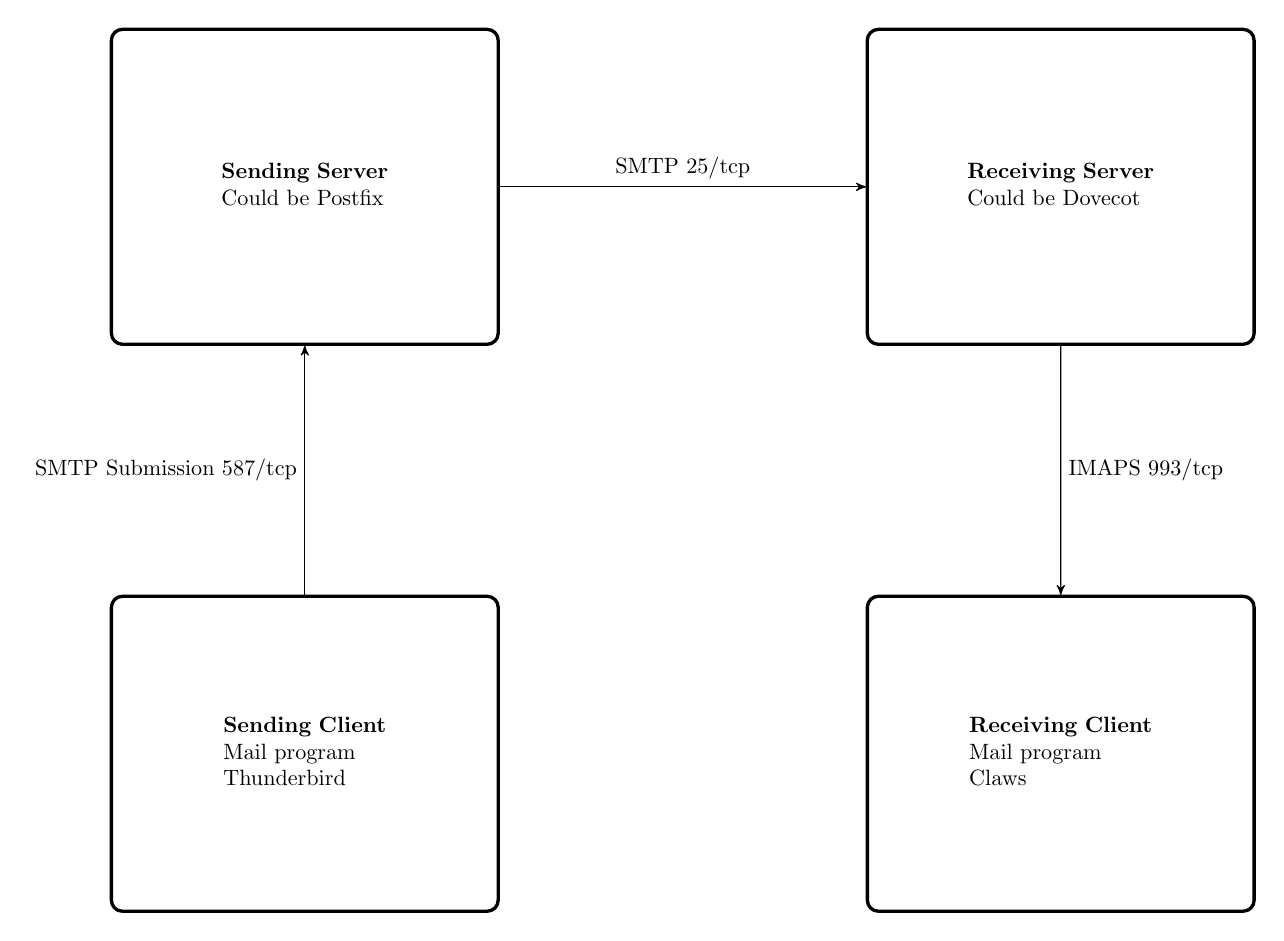
\begin{tikzpicture}[->,>=stealth',scale=0.8, transform shape]
  \newlength{\boxwidth}
  \setlength{\boxwidth}{6cm}
  \newlength{\boxheight}
  \setlength{\boxheight}{5cm}
  \newlength{\boxspace}
  \setlength{\boxspace}{12cm}

  % http://texample.net/tikz/examples/epc-flow-charts/

  % https://www.overleaf.com/learn/latex/LaTeX_Graphics_using_TikZ:_A_Tutorial_for_Beginners_(Part_3)%E2%80%94Creating_Flowcharts

   % Use previously defined 'state' as layout (see above)
   % use tabular for content to get columns/rows
   % parbox to limit width of the listing
   \node[state,text width=\boxwidth,minimum height=\boxheight] (SENDER)
   {\begin{tabular}{l}
   {\bf Sending Server}\\
      Could be Postfix
   \end{tabular}};

   %
   \node[state,         % layout (defined above)
    text width=\boxwidth,       % max text width
    minimum height=\boxheight,
    %yshift=2cm,                % move 2cm in y
    right of=SENDER,    % Position is to the right of QUERY
    node distance=\boxspace,    % distance to First node
    anchor=center] (RECEIVER)   % posistion relative to the center of the 'box'
   {%
   \begin{tabular}{l}
   {\bf Receiving Server}\\
Could be Dovecot
   \end{tabular}};

   \node[state,
    below of=SENDER,
    yshift=-8cm,
    anchor=center,
    minimum height=\boxheight,
    text width=\boxwidth] (THUNDERBIRD)
   {%
   \begin{tabular}{l}
   {\bf Sending Client}\\
    Mail program\\
    Thunderbird
   \end{tabular}
   };

   \node[state,
    below of=RECEIVER,
    yshift=-8cm,
    anchor=center,
    minimum height=\boxheight,
    text width=\boxwidth] (CLAWS)
   {%
   \begin{tabular}{l}
   {\bf Receiving Client}\\
    Mail program\\
    Claws
   \end{tabular}
   };
   % draw the paths and and print some Text below/above the graph
   \path
   (SENDER)     edge node[anchor=north,above]{SMTP 25/tcp} (RECEIVER)
   (THUNDERBIRD)        edge node[anchor=west,left]{SMTP Submission 587/tcp} (SENDER)
   (RECEIVER) edge node[anchor=east,right]{IMAPS 993/tcp }   (CLAWS);

\end{tikzpicture}
\end{center}


\slide{Email Software}

My recommendations are:
\begin{list2}
\item Sending mail with SMTP using Postfix
\item Receiving mail with IMAP using Dovecot
\end{list2}

I would NOT use these:
\begin{list2}
\item Exim - multiple Remote Code Execution in 2019, fatal security vulns \\
\url{https://www.exim.org/static/doc/security/}
\item OpenSMTPD has had some really strange vulnerabilities recently\\
\url{https://www.opensmtpd.org/security.html}
\item Dont use Sendmail - old and horrible
\end{list2}


Many more exist: \url{https://en.wikipedia.org/wiki/Comparison_of_mail_servers}

\slide{Postfix}

\hlkimage{3cm}{postfix-mouse.png}

\begin{quote}
  Postfix is a free and open-source mail transfer agent (MTA) that routes and delivers electronic mail.

It is released under the IBM Public License 1.0 which is a free software license. Alternatively, starting with version 3.2.5, it is available under the Eclipse Public License 2.0 at the user's option.[2]

Originally written in 1997 by Wietse Venema at the IBM Thomas J. Watson Research Center in New York, and first released in December 1998[3], Postfix continues as of 2020 to be actively developed by its creator and other contributors.
\end{quote}
Source: \url{https://en.wikipedia.org/wiki/Postfix_(software)}

Home page: \url{http://www.postfix.org/}


\slide{Dovecot}

\begin{quote}
Dovecot is an open-source IMAP and POP3 server for Unix-like operating systems, written primarily with security in mind.[3] Timo Sirainen originated Dovecot and first released it in July 2002. Dovecot developers primarily aim to produce a lightweight, fast and easy-to-set-up open-source email server.

The primary purpose of Dovecot is to act as mail storage server. Mail is delivered to the server using some mail delivery agent (MDA) and stored for later access with an email client (mail user agent, or MUA).
\end{quote}
Source: \url{https://en.wikipedia.org/wiki/Dovecot_(software)}

\begin{quote}
Dovecot is an open source IMAP and POP3 email server for Linux/UNIX-like systems, written with security primarily in mind. Dovecot is an excellent choice for both small and large installations. It's fast, simple to set up, requires no special administration and it uses very little memory.
\end{quote}
Home page: \url{https://www.dovecot.org/}




\slide{Securing Your Email Client}

\hlkimage{10cm}{thunderbird-enigmail-logo.png}

\begin{list2}
\item Security settings
\item Use TLS for SMTP
\item Use TLS for IMAPS
\item Disable loading of remote content, images, HTML parts, content, bugs, tracking
\item Disable sending version strings
\item Add plugins you need, but only those!
\end{list2}

Thunderbird mentioned as being one of the most popular email clients


\slide{CVE Details -- All software has errors! }
\hlkimage{19cm}{thunderbird-cves.png}

Source: {\footnotesize\url{https://www.cvedetails.com/product/3678/Mozilla-Thunderbird.html?vendor_id=452}}


\slide{Thunderbird Settings: }

\begin{quote}
Email messages can contain remote content such as images or stylesheets. To protect your privacy, Thunderbird does not load remote content automatically, but instead shows a notification bar to indicate that it blocked remote content.
\end{quote}

\begin{list2}
\item Privacy and security settings\\{\footnotesize \url{https://support.mozilla.org/da/products/thunderbird/privacy-and-security-settings}\\
\url{https://support.mozilla.org/en-US/products/thunderbird/privacy-and-security-settings}}
\item Previously you could override the User-Agent setting, setting it empty:\\
Does not work anymore
\url{https://bugzilla.mozilla.org/show_bug.cgi?id=1114475}
\item GPG and Enigmail for OpenPGP suppoprt - encrypted email\\
\url{https://support.mozilla.org/en-US/kb/digitally-signing-and-encrypting-messages}
\end{list2}

\slide{Claws Security Settings}

In my mail application there are other settings you can play with:

\begin{list2}
\item[\faCheck] Render HTML messages as text
\item[\faCheck] Use secure file deletion if possible
\item[\faCheck] Never send Return Receipts\\
When you receive a message that requests a Return Receipt a notification area is shown just above the message view. You can either use the 'Send receipt' button, or ignore the request - no receipts are sent automatically.
\item[\faSquareO] Automatically display attached images
\item[\faSquareO] Display images inline
\item[\faSquareO] Add user agent header -- don't
\end{list2}

BTW my mail client is not perfect either:\\{\footnotesize
\url{https://www.cvedetails.com/vulnerability-list/vendor_id-12415/Claws-mail.html}}


\slide{Advanced: Run your mail client in a VM}

\hlkimage{10cm}{claws-email.png}

I run my email client in a VM, which can only connect to my mail server and my printer

\begin{alltt}\footnotesize
[hlk@dom0 ~]$ qvm-firewall Mailreader
NO  ACTION  HOST             PROTOCOL  PORT(S)  SPECIAL TARGET  ICMP TYPE  EXPIRE  COMMENT
0   accept  192.0.222/32  tcp       993      -               -          -       -
1   accept  192.0.222/32  tcp       587      -               -          -       -
2   accept  10.0.42.13/32    tcp       515      -               -          -       -
3   drop    -                -         -        -               -          -       -
[hlk@dom0 ~]$
\end{alltt}




\slide{Unbound and NSD}

\begin{quote}
Unbound is a validating, recursive, caching DNS resolver. It is designed to be fast and lean and incorporates modern features based on open standards.

To help increase online privacy, Unbound supports DNS-over-TLS which allows clients to encrypt their communication. In addition, it supports various modern standards that limit the amount of data exchanged with authoritative servers.
\end{quote}

\link{https://www.nlnetlabs.nl/projects/unbound/about/}

My preferred local DNS server, and NSD is my preferred authoritative DNS server

Also check out uncensored DNS and his DNS over TLS setup!\\
Even has pinning information available:\\ {\small\link{https://blog.censurfridns.dk/blog/32-dns-over-tls-pinning-information-for-unicastcensurfridnsdk/}}


\slide{Email security -- Goals}

\begin{list2}
\item SPF Sender Policy Framework\\ {\footnotesize\link{https://en.wikipedia.org/wiki/Sender_Policy_Framework}}
\item DKIM DomainKeys Identified Mail\\
{\footnotesize\link{https://en.wikipedia.org/wiki/DomainKeys_Identified_Mail}}
\item DMARC Domain-based Message Authentication, Reporting and Conformance\\
{\footnotesize\link{https://en.wikipedia.org/wiki/DMARC}}
\item Use them all
\end{list2}

A huge part of email security is ensuring our domains are not abused in spoofing attacks, and spam



\slide{Sender Policy Framework (SPF)}

\begin{alltt}
 $ host -t TXT zencurity.com
 zencurity.com descriptive text "v=spf1 a mx mx:kramse.dk -all"
\end{alltt}

\begin{quote}\footnotesize
Sender Policy Framework (SPF) is an email authentication method designed to detect forging sender addresses during the delivery of the email.[1] SPF alone, though, is limited only to detect a forged sender claimed in the envelope of the email which is used when the mail gets bounced.[1] {\bf Only in combination with DMARC can it be used to detect the forging of the visible sender in emails} (email spoofing[2]), a technique often used in phishing and email spam.

SPF allows the receiving mail server to check during mail delivery that a mail claiming to come from a specific domain is submitted by an IP address authorized by that domain's administrators.[3] The list of authorized sending hosts and IP addresses for a domain is published in the DNS records for that domain.
\end{quote}

Source:\\{\footnotesize
\link{https://en.wikipedia.org/wiki/Sender_Policy_Framework}}


\slide{DomainKeys Identified Mail (DKIM)}

\begin{quote}
DomainKeys Identified Mail (DKIM) allows the receiver to check that an email claimed to have come from a specific domain was indeed authorized by the owner of that domain.[1] It achieves this by affixing a digital signature, linked to a domain name, to each outgoing email message. The recipient system can verify this by looking up the sender's public key published in the DNS. A valid signature also guarantees that some parts of the email (possibly including attachments) have not been modified since the signature was affixed.[2] Usually, DKIM signatures are not visible to end-users, and are affixed or verified by the infrastructure rather than the message's authors and recipients.
\end{quote}

Source: \\{\footnotesize
\link{https://en.wikipedia.org/wiki/DomainKeys_Identified_Mail}}

\slide{Domain-based Message Authentication (DMARC)}

\begin{quote}\footnotesize
DMARC (Domain-based Message Authentication, Reporting and Conformance) is an email authentication protocol. It is designed to give email domain owners the ability to protect their domain from unauthorized use, commonly known as email spoofing. The purpose and primary outcome of implementing DMARC is to protect a domain from being used in business email compromise attacks, phishing emails, email scams and other cyber threat activities.

Once the DMARC DNS entry is published, any receiving email server can authenticate the incoming email based on the instructions published by the domain owner within the DNS entry. If the email passes the authentication it will be delivered and can be trusted. If the email fails the check, depending on the instructions held within the DMARC record the email could be delivered, quarantined or rejected.

DMARC extends two existing mechanisms, Sender Policy Framework (SPF) and DomainKeys Identified Mail (DKIM).
\end{quote}
DMARC Domain-based Message Authentication, Reporting and Conformance\\
Source: \\{\footnotesize
\link{https://en.wikipedia.org/wiki/DMARC}}


\slide{DMARC for non-sending Domains}
If you have domains that \emph{never send email} then add the following SPF and DMARC to avoid misuse.

from my own DSN template for \emph{parked domains}:
\begin{alltt}
gdns.template   v=spf1 -all     43200
_dmarc.gdns.template    v=DMARC1; p=reject;     43200
\end{alltt}


\slide{You Don't Have to Do It Alone}

%\hlkimage{}{}

\begin{quote}
Self-hosting does not mean doing everything yourself from scratch.
There is a thriving ecosystem of communities, cooperatives, and associations
that run shared infrastructure for their members — combining the benefits
of self-hosting with shared operational responsibility.
\end{quote}

\begin{list2}
\item Associations and cooperatives can pool resources — shared hardware,
shared skills, shared on-call burden
\item Members retain control and trust in the people running the service,
rather than a faceless corporation
\item A great middle ground between full DIY and surrendering to Big Tech
\item The following examples show real organisations doing exactly this —
each with different scope, values, and technical approaches
\item They may also inspire you to start something similar in your own community,
workplace, or interest group
\end{list2}


\slide{Some Examples: Fripost - The Free Email Association}

\begin{quote}{\bf \large
Fripost - The Free Email Association}

Technology has never been neutral. The ownership structure of technology companies and their endeavour for profit ensures that usage of their services for work and communication will never be free.

At the same time, only a fraction of the everyday Internet users have knowledge and resources enough to create free alternatives on their own. The question is also: What can reasonably be expected from an average user in terms of engagement in their privacy and freedom?

For any one individual, the goal of user freedom may be unattainable. Together, we can move mountains.

We are proud to present the Association for Free Email, Fripost. Fripost has since late 2010 delivered a free and reliable email service, with a distributed network of servers.
\end{quote}

Source:  \link{https://fripost.org}



\slide{Some Examples: data.coop}

\begin{quote}{\bf \large
Velkommen til data.coop}

data.coop er et kooperativ, som ejer og driver en digital infrastruktur for medlemmerne. Vores grundlæggende formål er at passe på medlemmernes data.

Vores kerneprincipper er:

Privatlivsbeskyttelse
\begin{list2}
\item Vi er fælles om at beskytte vores data. Vi deler dem ikke for profit. Dine data transmitteres krypteret på nettet.
Kryptering
\item Vi tilbyder løsninger, der er sikre og grundigt deklarerede.
Decentralisering
\item Vores services snakker gerne sammen med andre decentrale services på nettet.
Zero-knowledge
\item Når det er muligt, sørger vi for, at systemadministratorer rent teknisk ikke kan tilgå medlemmernes data.
\end{list2}

Ud fra de kerneprincipper vil vi med tiden udbyde onlinetjenester til medlemmerne. Hovedtanken er, at vi som udgangspunkt stoler mere på hinanden end på “de store” som f.eks. Google, Microsoft eller Facebook.

\end{quote}

Source:  \link{https://data.coop}

\slide{Some Examples: kantree -- buy from better companies}

\begin{quote}
At Kantree, we believe in collaboration, transparency and trust.
As a workers cooperative (100\% employee-owned company), these values are deeply rooted.
They are reflected in our products and in the relationship we build with each customer.

...

While a lot of {\bf competitors are focusing on AI, we believe human interactions are the actual missing piece} to making digital collaboration tools better suited for the future of work. We should not strive to eliminate the human element from our tools, but rather take advantage of our collective intelligence.

...
More autonomy implies a deeper involvement. It requires transparency to ensure a clear vision of the situation and of the objectives. It also requires processes which are adapted to each teams and which can evolve through time.

{\bf These believes combined with our values led us to create Digicoop, the company behind Kantree.}

%We are a French team, passionate about technology, the web and what it can bring to society. We are using our experience to build great products that we hope have a positive impact.

%{\bf Because we really stand behind our values, Digicoop is a worker cooperative fully owned by its employees.} A company is made of people and we think giving every one of them a stake in it allows them to have a meaningful impact on its future.
\end{quote}

Source:  \link{https://kantree.io/about}


\slide{Things We Didn't Cover: File Sync and Collaboration}

%\hlkimage{}{}

\begin{quote}
Replacing cloud storage and office collaboration tools is very achievable
with self-hosted open source software
\end{quote}

\begin{list2}
\item {\bf Nextcloud} — the most complete self-hosted collaboration platform:
files, calendar, contacts, video calls, office documents, and more \link{https://nextcloud.com}
\item {\bf Syncthing} — decentralised file synchronisation between your own devices,
no server required \link{https://syncthing.net}
\item {\bf Seafile} — fast, reliable file sync with a focus on performance and simplicity \link{https://seafile.com}
\item {\bf OnlyOffice} and {\bf Collabora Online} integrate with Nextcloud to provide
browser-based editing of Word, Excel, and PowerPoint compatible documents
\item {\bf Cryptpad} — end-to-end encrypted collaborative documents, spreadsheets,
and kanban boards \link{https://cryptpad.fr}
\item All of these run well in Docker containers — a \verb+docker-compose.yml+ and
an NGINX reverse proxy is usually all you need to get started
\end{list2}


\slide{Things We Didn't Cover: Communication and Messaging}

%\hlkimage{}{}

\begin{quote}
Microsoft Teams, Slack, and Zoom dominate workplaces —
but self-hosted alternatives exist for all of them,
with better privacy and no per-seat licensing costs.
\end{quote}

\begin{list2}
\item {\bf Mattermost} — open source Slack alternative, self-hosted,
with threads, channels, and integrations \link{https://mattermost.com}
\item {\bf Matrix / Element} — federated, encrypted messaging and team chat;
run your own homeserver with Synapse or Conduit \link{https://matrix.org}
\item {\bf Jitsi Meet} — self-hosted video conferencing, no account required,
works in the browser \link{https://jitsi.org}
\item {\bf Rocket.Chat} — team messaging with video, file sharing,
and a large plugin ecosystem \link{https://rocket.chat}
\item {\bf XMPP} — the original open federated messaging protocol, still widely used,
clients include Conversations (Android) and Gajim (desktop)
\item Federation matters: Matrix and XMPP allow communication across different servers —
you are not locked into a single provider or instance
\end{list2}


\slide{Things We Didn't Cover: Monitoring, Passwords, and More}


\begin{list2}
\item {\bf Monitoring} — {\bf LibreNMS} for network monitoring \link{https://librenms.org},
{\bf Grafana} + {\bf Prometheus} for metrics and dashboards \link{https://grafana.com}
\item {\bf Password management} — {\bf Bitwarden} offers an official self-hosted server
\link{https://bitwarden.com}; {\bf Vaultwarden} is a lightweight community reimplementation
in Rust, compatible with all Bitwarden clients and easier to run on modest hardware
\link{https://github.com/dani-garcia/vaultwarden}
\item {\bf DNS filtering} — {\bf Pi-hole} block ads and
tracking domains network-wide via DNS \link{https://pi-hole.net}
\item {\bf Git hosting} — {\bf Gitea} or {\bf Forgejo} provide a lightweight self-hosted
GitHub alternative for code and documentation \link{https://forgejo.org}
\item {\bf Home automation} — {\bf Home Assistant} runs locally and keeps your smart
home data off vendor clouds \link{https://www.home-assistant.io}
\item The self-hosting community maintains {\bf Awesome-Selfhosted} —
a curated list of hundreds of options \link{https://awesome-selfhosted.net}
\end{list2}


\slide{Things We Didn't Cover: Client Operating Systems}

\begin{list2}
\item {\bf Debian} — rock-solid, well-supported Linux desktop and laptop OS;
what we use at Zencurity for workstations \link{https://www.debian.org}
\item {\bf Ubuntu} — Debian-based, more beginner-friendly, large community and
good hardware support; a natural first step from Windows or macOS \link{https://ubuntu.com}
\item {\bf Fedora} — Red Hat sponsored, cutting-edge packages, good for developers \link{https://fedoraproject.org}
\item {\bf Linux Mint} — often recommended as the most approachable desktop Linux
for people switching from Windows \link{https://linuxmint.com}
\item {\bf Qubes OS} — security through compartmentalisation; runs each application
or context in a separate VM (qube); not for everyone, but very powerful for
high-security workstations — used at Zencurity \link{https://www.qubes-os.org}
\item All of the above are free, open source, and run well on modest hardware —
including older laptops that Windows 11 refuses to support
\end{list2}

\slide{Conclusion: Take Control, Take Responsibility}

%\hlkimage{}{}


Self-hosting is not for everyone — but for those who choose it,
it offers genuine independence, real learning, and ownership of your data


\begin{list2}
\item {\bf Start small} — a single VPS with NGINX and UFW is already self-hosting
\item {\bf Use open standards} — OCI images, open protocols, open formats keep your options open
\item {\bf Version control everything} — if it is not in Git, it does not exist
\item {\bf Security is not optional} — firewalls, TLS, patching, and backups from day one
\item {\bf You are on call} — know this going in, and plan for it
\item {\bf Communities help} — cooperatives, associations, and friendly sysadmins
share the burden and the knowledge
\item {\bf Digital sovereignty is a journey} — every service you move away from Big Tech
is a step toward independence
\end{list2}


\myquestionspage


\end{document}
